\documentclass[onecolumn, draftclsnofoot,10pt, compsoc]{IEEEtran}

%slightly modified from stackoverflow @ https://tex.stackexchange.com/questions/200437/numbering-sections-subsections-etc-manually
%code block below allows for references to function as a section instead of a chapter
\makeatletter
\renewenvironment{thebibliography}[1]
{\subsection{References}
	\@mkboth{\MakeUppercase\bibname}{\MakeUppercase\bibname}%
	\list{\@biblabel{\@arabic\c@enumiv}}%
	{\settowidth\labelwidth{\@biblabel{#1}}%
		\leftmargin\labelwidth
		\advance\leftmargin\labelsep
		\@openbib@code
		\usecounter{enumiv}%
		\let\p@enumiv\@empty
		\renewcommand\theenumiv{\@arabic\c@enumiv}}%
%	\sloppy
	\clubpenalty4000
	\@clubpenalty \clubpenalty
	\widowpenalty4000%
	\sfcode`\.\@m}
{\def\@noitemerr
	{\@latex@warning{Empty `thebibliography' environment}}%
	\endlist}
\makeatother

\usepackage{graphicx}
\usepackage{url}
\usepackage{setspace}
\makeindex
\usepackage{geometry}
\usepackage{float}
\usepackage{caption}

\geometry{textheight=9.5in, textwidth=7in}

% 1. Fill in these details
\def \CapstoneTeamName{		Wheelchair Data Collection Team}
\def \CapstoneTeamNumber{		4}
\def \GroupMemberOne{			Marie Bomber}
\def \GroupMemberTwo{			Aaron Leondar}
\def \GroupMemberThree{			Hadi Rahal-Arabi}
\def \CapstoneProjectName{			Robotic Wheelchair Data Collection and Analysis}
\def \CapstoneSponsorCompany{	Oregon State University}
\def \CapstoneSponsorPerson{	Matthew William Shuman	}

% 2. Uncomment the appropriate line below so that the document type works
\def \DocType{	%Problem Statement
				%Requirements Document
				%Technology Review
				%Design Document
					Midterm Progress Report
				}
\bibliographystyle{ieeetran}	
\newcommand{\NameSigPair}[1]{\par
\makebox[2.75in][r]{#1} \hfil 	\makebox[3.25in]{\makebox[2.25in]{\hrulefill} \hfill		\makebox[.75in]{\hrulefill}}
\par\vspace{-12pt} \textit{\tiny\noindent
\makebox[2.75in]{} \hfil		\makebox[3.25in]{\makebox[2.25in][r]{Signature} \hfill	\makebox[.75in][r]{Date}}}}
% 3. If the document is not to be signed, uncomment the RENEWcommand below
%\renewcommand{\NameSigPair}[1]{#1}

%%%%%%%%%%%%%%%%%%%%%%%%%%%%%%%%%%%%%%%
\begin{document}
\begin{titlepage}
    \pagenumbering{gobble}
    \begin{singlespace}
        \hfill 
        % 4. If you have a logo, use this includegraphics command to put it on the coversheet.
        %\includegraphics[height=4cm]{CompanyLogo}   
        \par\vspace{.2in}
        \centering
        \scshape{
            \huge CS Capstone \DocType \par
            {\large 16 February 2018}\par
            \vspace{.5in}
            \textbf{\Huge\CapstoneProjectName}\par
            \vfill
            {\large Prepared for}\par
            \Huge \CapstoneSponsorCompany\par
            \vspace{5pt}
            {\Large\NameSigPair{\CapstoneSponsorPerson}\par}
            {\large Prepared by }\par
            Group\CapstoneTeamNumber\par
            % 5. comment out the line below this one if you do not wish to name your team
            \CapstoneTeamName\par 
            \vspace{5pt}
            {\Large
                \NameSigPair{\GroupMemberOne}\par
                \NameSigPair{\GroupMemberTwo}\par
                \NameSigPair{\GroupMemberThree}\par
            }
            \vspace{20pt}
				\begin{abstract}
This document serves to function as a progress report on the ROS Test Controller. The document is broken up into multiple sections. The first is a re-introduction into the project’s purposes and goals for the uninitiated. Following this introduction, there are several perspectives on the project’s current status, next steps, and issues with development. The document is not independent, and there is some technology referenced that will require the reading of previous specifications documents for the Wheelchair Data Collection Project.
				\end{abstract} 
        }   
    \end{singlespace}
\end{titlepage}
\newpage
\pagenumbering{arabic}
\tableofcontents
%\listoffigures
%\listoftables
\clearpage


\section{Introduction}
%Project purposes and goals go here
\subsection{Project Purpose}
Robotic testing, more specifically robot data collection, has been an area that, while well-documented, is not well optimized. The time and amount of commands needed in order to set up a ROS environment to record test data is quite a lot. For example, to set up an environment to record tests with Project Chiron, around 10+ commands must be inputted in several different windows. The purpose of this project is to create an interface that is able to make the whole process of collecting data using ROS easier, from setup to data collection to data playback and storage. If the process of setting up tests to be able to collect data is made easier and made more streamlined, then it opens the door for even people who know nothing about ROS to still be able to run tests and collect data. It has the ability to not only satisfy research needs, but also can be useful in everyday situations, where any random person is able to use it effectively and run the same kinds of tests that a researcher can run.
\subsection{Project Goals}
The goals of this project are to simplify all the ROS connection commands and data collection setup into one simple interface. Doing so allows the entire process to be streamlined and eliminates the need to remember the list of complex commands needed to start recording manually. If the complexity is able to be taken out of the data recording process, then that means an expert in ROS will no longer have to be a requirement in order to set up and record a test. A researcher has the potential to hire a freshman undergraduate who knows little to nothing about robots, ROS, or even Computer Science, and the freshman will be able to create and run tests for the researcher. This allows the researcher to not have to worry about the testing aspect of their research, and can focus their efforts on more complicated research, as well as focusing on using the data that was collected and applying it to their research. If the goal of creating a simplified interface can be met, then the interface can be applied to more than just the project here. It has the potential to be released as open-source software to be used with any robot that runs ROS.

\section{Marie's Individual Section}
\subsection{Project Status}
The ROS Test Controller project has evolved quite a bit from the original inception in at the beginning of fall term. What was originally conceived as a single use application, designed to meet the needs of our client as he collected testing data for Project Chiron, has evolved into a reusable interface to assist users of ROS design and run robotics tests. In addition, while we initially intended for the interface to run entirely in Python (as we expected the primary users to be more comfortable in Python and therefore, enhance maintainability) we have instead shifted into a NodeJS based web application. This primary shift came about due to Python having limited libraries for using SSH, the primary method of communicating with a robot using ROS. While the specifics of the connection issues will be addressed the next section, suffice to say the shift from a Python solution to a NodeJS solution broke a nearly two week block in project progress. 

As of February 14th, we were able to solve our connection issue by moving to a web application and will be testing the ‘bare-bones’ solution to our client on Monday the 19th. This mini-version of the application will focus on the client’s primary need, an interface that requires only one or two clicks to start, record and end a test.

\begin{figure}[H]
	\centering
	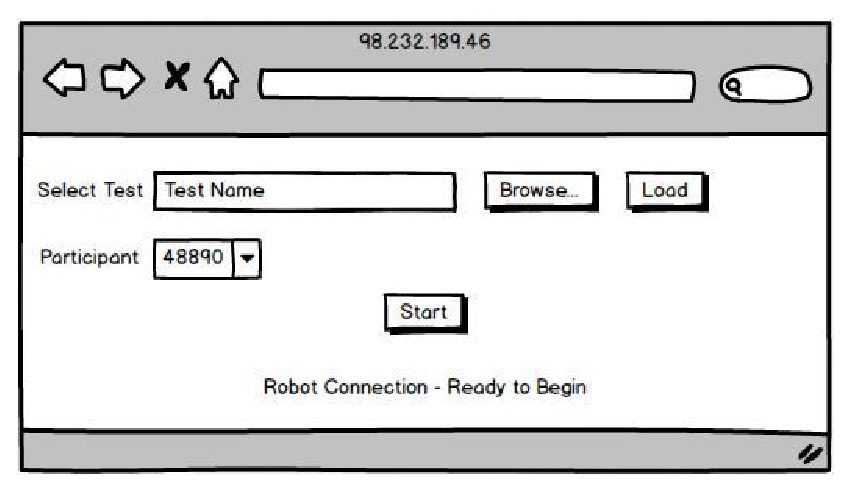
\includegraphics[scale=0.6]{BarebonesMockup.eps}
	\centering
	\caption{Mockup of 'Bare-Bones' interface}
\end{figure}

Currently, the client must have four terminals open and run 3 startup scripts before the robot is prepared to begin a test and then yet another command for the test to begin. This interface will automatically run the startup scripts for the client and transition beginning and ending a test to a single button click. Once we have successfully tested the ‘bare-bones’ solution, the client will be able to use the bare-bones solution while we expand the application. 

\subsection{Next Steps}
Once our application has been tested successfully, our next stage will be to add additional functionality to the interface. The core functionality of the solution can be split into three main stages. First, there is the 'run test' interface that we created in the first stage. Then there is creating new tests (so that the same interface can be used for multiple robots and test scenarios), last and least critical is the ability to view previous test results. This will expand the use of the interface to designing tests, recording an instance of a test and viewing of a previously recorded test.

While it has taken us six weeks to reach the first section of the interface, we are confident we will be able to deliver the final two sections in far less time. Our primary struggle when designing the application was not in individual components (such as creating a file storage method, or even running the ROS commands that were needed) or in getting each component to not only work together, but to work over an SSH interface. 

\subsection{Project Problems}
The primary issue we have encountered occurred shortly before we were to deliver our alpha version of the product to the client. Running a ROS test could be generalized into three stages, connect to the robot using SSH, run any startup scripts and then run the ROSbag command. Prior to the delivery date for our client, we had Python scripts to handle each stage of the test, as well as an interface that would act as the 'central command' for the interface. Each script had been tested on our remote server (that also functioned as a 'dummy' robot to enhance the parallels to a live environment) and were communicating smoothly between one another. Unfortunately, when we linked each component together and ran them via a remote SSH connection using Piminko, everything broke down. After considerable research, we discovered that the Python libraries we were using to set up and run our connection did not initialize environment variables that our script relied on. At this point, Hadi suggested that we move to a NodeJS approach. While we were reluctant to change gears so late (our initial delivery date was the 1st of February and it was the 31st of January), Hadi promised he would be able to prove that this approach would better fit both our client's needs as well as our own. 

With the shift to nodeJS, I took a more active role in the ROS communication portion of the project (previously, my primary role had been the filesystem, which was currently in a stable state). I was tasked with generating a bash script that Node could call when a request to record was received. Using a shell script mitigated our environment variable issues, but came with it's own concerns regarding relative or absolute paths of specific ROS commands. As of February 16th, our interface currently uses a hard coded path for the ROS calls, but as we move to a more general solution, this will have to change. 

\subsection{Interface Design}
Because a well designed UI was a priority for our client, Aaron and I have undertaken the ROS Test Controller as our primary project for the Intro to Usability Design class this quarter. This has allowed us additional time to both interview our client for usability research as well as dedicate energy into designing an streamlined interface. While the project is still in it's 'bare-bones' stage (with the UI for Bare-bones coming on Sunday the 18th), we have a strong understanding on the 'flow' of each individual view the client (and future users) will encounter. While not every window has a mockup yet, each window has at least been designed and individual components have been conceived. 

\begin{figure}[H]
	\centering
	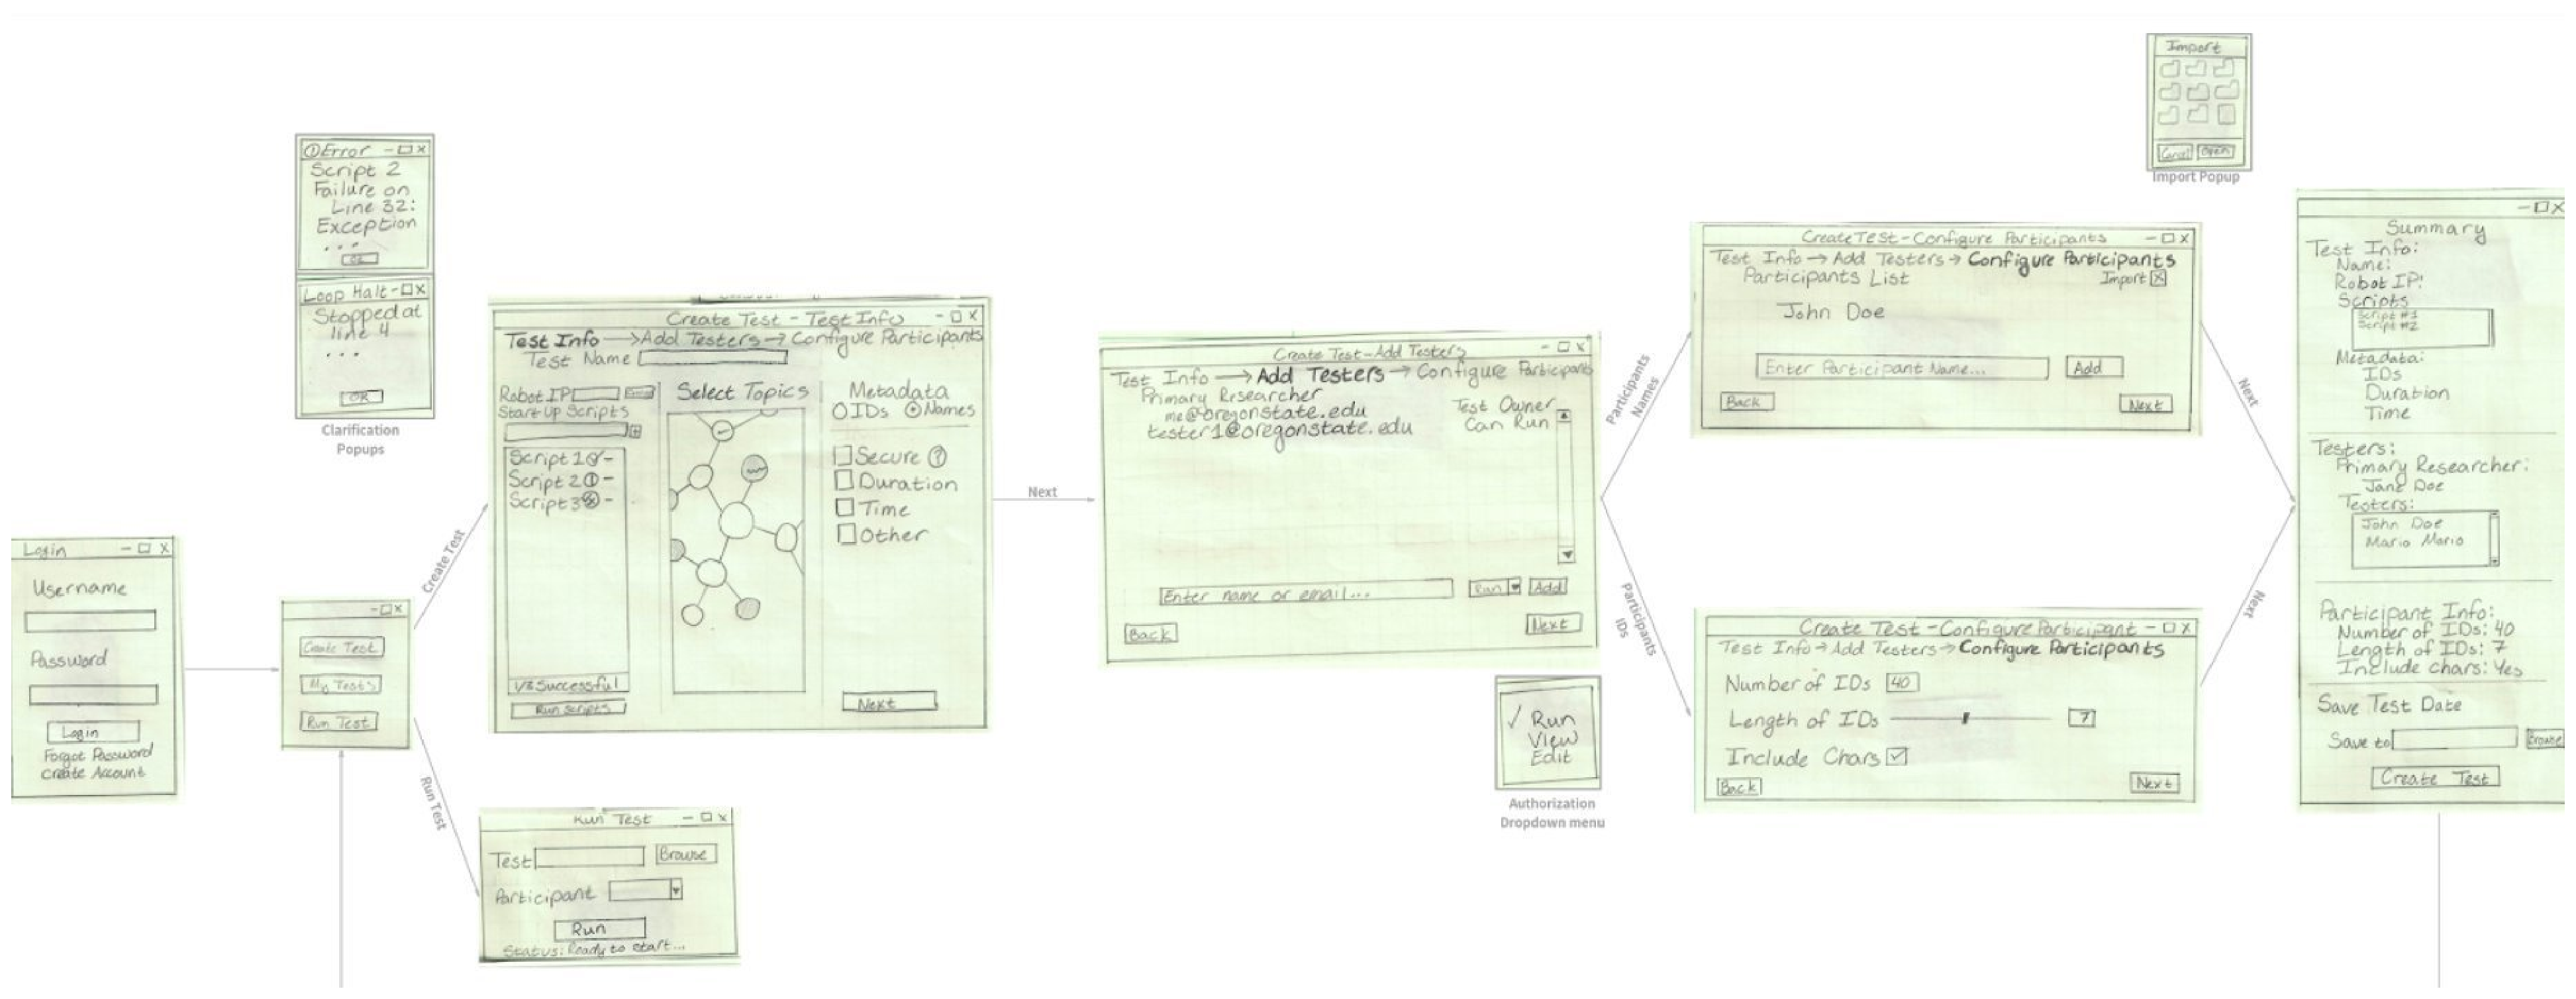
\includegraphics[scale=0.25]{Prototype.eps}
	\caption{Figure 2: Prototype for two modes of ROS Test Controller}
\end{figure}

While the 'My Tests' section is currently still under design, the components within (edit, view and delete tests) all fall under stretch goals of the project and can be removed should we run out of time. These current windows represent the primary 'flow' of creating a new test, including naming the test, connecting to the robot, testing startup scripts, selecting what 'topics' to record (in other words, what data, such as camera feeds or wheel location information) and what non-robot data to include in an individual user test.

\section{Aaron's Individual Section}

\subsection{Current Status}
We have just completed a bare-bones alpha of our interface in Node.js. We originally started in Python, but ran into several problems that impeded progress. The only parts of our project that are actually in working condition is using the interface to connect to the wheelchair robot, launch the pre-determined roslaunch files that were given to us by our client, then run the recording function to collect data in a bag. The bag is then stored in specific folder on the Robot's NUC and can be retrieved later. Its functionality right now is basically that it solely functions with the Project Chiron Permobil wheelchair, and no other robot that runs ROS.

\subsection{What's Left To Do}
The main goal to focus on now is to expand functionality to a general use-case, so that the interface can be used with any robot that is able to run ROS, not just the Project Chiron wheelchair. The functions that will need to be added includes the ability to create new tests, select certain topics to record from a list, save tests so they can be run again later without having to waste time inputting all the parameters again, and divide users into researchers, who have a lot more freedom with the interface, and testers, who just have freedom to create and record tests. Also, other tasks to work on are making the interface look appealing and efficient, so that users will be able to learn its functions very quickly and will be able to remember those actions. Finally, the other important task is to document everything about our interface, from how it works with connectivity and recording, to how to run a sample test, in order to be able to release it in the future as an open-source project.

\subsection{Problems/Solutions}
We had problems that needed to be addressed since finals week of Fall term. During that week, we held a meeting with our client in order to get some hands-on experience with the Project Chiron wheelchair, so that we knew what we were working with. The problems that cropped up due to that meeting were that we were approaching the project slightly differently than our client wanted. We were designing the interface to exclusively with the Project Chiron Permobil wheelchair, however our client wanted something that used more of a general use case. So we had to redesign our requirements and design documents to not only include the requirements the Project Chiron wheelchair, but also include requirements for a general use case, so that the interface can be run on any robot that is able to run ROS. Another problem that needed to be addressed and fixed due to that meeting was that we needed to separate the two different types of users who would use this interface: the researchers and the testers. We originally planned the interface to behave the same no matter who was accessing it. The problems with this method became apparent in our meeting because testers who would use the interface would have access to all of the data collected, and that is something that we do not want to happen. So to solve that problem we had to split the users into the researchers and testers. Researchers would have freedom to create and record tests, be able to play back tests, and most importantly, be able to export the data collection to be used for various research projects/purposes. In contrast, testers should not have nearly that much freedom, and should only be able to create new tests and to be able to actually record the tests. The testers should not have any access to any of the actual information that is recorded in the bag file. Due to these problems that came to light because of our meeting, we had to edit our Requirements and Design documents in January, and get them re-verified and re-approved by our client before we could actually start development. Possibly the biggest problem that we have run into since starting this project has been being able to run a ROS environment remotely through ssh. Normally, when setting up and running a ROS environment, it is done within the command line on the same machine that is running the interface. However, because our interface aims to reduce the number of commands that the user has to input, the problem arises that suddenly we have run all of the ROS commands through python code, as opposed to just through the command line, and Python does not like that. Python already does not handle ssh connections well, preferring instead to use ftp, and when python is used to ssh into a robot, the source environment used to run ROS is missing. In short, Python being used to ssh into a robot and run ROS commands does not work well if a command line is not present, which it should not be, otherwise our interface would be completely pointless. The latest problem we have had to deal with has been switching away from Python to a language that supports what we are trying to do with our interface better, which we found to be Node.js. Only one member of our group has ever had experience with Node, and it was a decision that was made a couple weeks before the mid-way point in the term, so it was something that had to be implemented very quickly. However, it is a decision that we think will be more beneficial in the long run, as it will make adding additional features easier in the future, and will make the code way less messy and be way more functional.

\subsection{Relevant/Interesting Information}

What's interesting about our interface is that it is made in Node.js, which is a language that none of the members of our group have any significant experience working in, and two of us have absolutely zero experience working in it. Also, because our Python interface was determined to be bad and was scrapped so close to the mid-term, our bare bones Node interface had to be written in a matter of a couple of days, compared to our Python interface which took about 3-4 weeks.

\section{Hadi's Individual Section}
\subsection{Project Status}
\subsubsection{Alpha Specification}
The Ros Test Controller Alpha has been developed. 
The alpha contains only the critical functionality required to allow a user to record a rosbag. The project has pivoted from a python app to a nodejs server, which allows us to develop the application as a series of API endpoints and calls. The http calls are handled by nodejs-express, and This allows us to split the project into a set of conceptual microservices. These API methods interact with ROS by making calls to the node “exec” library, typically by calling a bash script on the system. The inputs to the API methods are not sanitized, meaning the node server host is vulnerable to any user who has access to the interface. However, since this project is intended to operate only on a local network, this security risk is significantly minimized.\\
Templating for this application is done in express-handlebars, which allows for many different views of the interface to be created under a similar structure, in very limited development time. Visually, the alpha contains only two elements, a text input section for the ID of a data collection test participant, and a “record” button.\\
The alpha interface includes a single page, in which a tester can enter a participants ID number and record the ROSbag of his trial. The record button simply passes along the relevant information to the node server in a GET request. Although this is less secure than a post request, this is functionally irrelevant in the scope of alpha.

\subsubsection{Project Management}
Project management and communication in the status quo is largely handled in Slack, although there is a set of tasks in waffle.io. These tasks are intended to be completed with as part of an agile workflow. Marie handles the management of these tasks, by keeping up to date on the status of the project, and notifying the team when a task needs to be completed, or when a task’s priority has changed. While there have been issues with delivery of the alpha, which are discussed below, they are related to failures in architecting the software effectively, and not in the management of the project.

\subsubsection{Shifts in Responsibility}
The original set of responsibilities was contingent on creating a python application, as Aaron was intended to research methodologies for connecting a remote interface to the Robot Operating System. Since these connections are handled trivially with HTTP/REST calls, Aaron has shifted his focus to interface design and user-experience. This covers my old responsibilities on the python demo, allowing me to shift to writing the API methods for the interface. Marie continues to operate in her role as project manager, and she also works with Aaron on writing the ROS system calls that are passed from the node server.

\subsection{Next Steps}

\subsubsection{Upgrades in Beta}
The beta will contain input sanitation to prevent hijacking of the node server host. This will allow the project to be safely shared to the ROS community without creating several extremely vulnerable robot hosts. The beta will include a more visually appealing interface that allows for more complicated interactions with the user. This specifications for this visual interface have been provided directly by the client via email. The beta will also contain more methods to anonymize the user data stored with the bag data file.\\
Beta will need to contain significantly more robust error-reporting, as the alpha only reports issues during a full crash. Beta should notify the user of any issues and contain more unit tests to help guarantee the successful operation of the application.\\
The Ros Test Controller Beta should contain the necessary documentation for developers to extend the set of services provided by the API hosted by the node server. This will allow future (and current) development to be a more streamlined and standardized process. 

\subsubsection{Expo Preparation}
The data collection project is not independently visually interesting, as it largely was a project of web-calls and API design. This means that the expo preparation will need to be significant to find ways to keep the interest of the attendees. \\
The team is considering finding a physical robot that can be tracked during expo, with the results displayed in real-time. However, this would require significant extensions to the alpha, for which the development has not been planned. The client has approved these extensions in a meeting during the fall term, so the team is at liberty to pursue this avenue if given the time and prioritization. \\
If a robot is not obtained, we must plan another way to engage the attendees at expo, as the interface itself is not visually exciting, and the underlying technology is only relevant and interesting to web developers. A possible method of doing so is to create a simple virtual robot (turtlebot) which can be controlled using an Xbox controller, and recording its movements. With the right approach, this can be appealing to the attendees at expo as an experience similar to playing a video game.


\subsection{Project Problems}

\subsubsection{Stalling on Python Demo}
While the capstone alpha was due this week, we had intended to deliver it to the client two weeks ago. However, this was delayed due to architecture issues. The team had planned to develop the alpha in python, using an emulated ssh terminal connection to make calls to ROS on the NUC. However, emulating an SSH connection does not actually create a shell, which contains the necessary environment variables for ROSbag to interact with the ROS core. We scrapped this structure but lost multiple weeks of development time creating it.

\subsubsection{Workflow Issues}
There have been some issues working under an agile workflow. While the project management has been effective, unanticipated roadblocks stalled our development, which in turn has effectively ended the intended development cycle. We will need to re-write many of our tasks in the upcoming weeks to fit our new understanding of the project and its goals.

%\bibliography{ProjectBib}

\end{document}
